


\section{Accretion \label{sect:accretion}}

Accretion is the defining characteristic of star formation. It is through accretion that stars build up mass, it is through accretion that they accumulate angular momentum, and it is probably through magnetic connection between disk and accretion column that at least some part of their angular momentum is lost. Once accretions stops, stars continue to evolve, but on much longer time scales, e.g., through stellar winds, which change the mass, chemical composition, and angular momentum of a star over Gyr time-scales.

Today it is widely accepted that the accretion in T Tauri stars is magnetically funneled \citep{Hartmann_2016}. The accretion disk does not reach down to the stellar surface. Instead, it is truncated at a few stellar radii close to the radius where the disk co-rotates with the central star. While magnetic fields of young stars can be complex with the near-field dominated by higher order multipoles, the dipole moment is assumed to dominate at distances of a few stellar radii\footnote{There seems to be an evolution of magnetic field strength and geometry, where the strength of the dipole component decreases with the depth of the convective zone \cite{2012ApJ...755...97G,2019A&A...622A..72V}, but even if higher magnetic moments are stronger at the stellar surface, the dipole typically dominates at the inner disk edge.}. These (dipole) magnetic field lines couple the star with the inner disk and disk material, ionized by the UV and X-ray radiation from the star, is forced to follow the field lines. As it falls in, gravity accelerates the matter to almost free-fall velocity until it hits the surface where a strong shock develops \cite{Shu_1994}, and the post-shock plasma is so hot that it cools primarily through X-ray emission.  Depending on the height and geometry, those X-rays may or may not be visible, but the shock certainly heats the surrounding photosphere, which causes bright UV emission and optical veiling (a strong continuum that makes phtotospheric emission lines appear weaker than in a non-accreting star). To better understand the accretion geometry in CTTS, we first discuss the accretion stream and the locations of the footpoints. Then, we describe simple 1D accretion shocks before we turn to more detailed observations and models.

\subsection{The accretion stream and its foot points}
\label{sect:accretionsrteam}
The accretion stream is initially cool ($\log T\sim3-4$), because it is fed by inner disk material; it heats up as mass accelerates and comes closer to the star. The most prominent tracers are the strong and complex hydrogen emission lines. In particular H$\alpha$ is usually optically thick and often shows red-shifted absorption components compatible with near free-fall velocity \cite[e.g.][]{2000AJ....119.1881A}, and varies over time scales of hours \cite{dupree_2012}. Since many emission lines, however, do not vary with the stellar rotation period, it is likely that the inner disk is more important for accretion than the anchor point on the stellar surface \cite{2021A&A...649A..68S}. 

The structure of the stellar magnetic field can be probed by Zeeman-Doppler imaging and, using certain assumptions, those fields can be extrapolated out to the inner disk edge where the dipole component usually dominates the coupling of the star with the accretion disk; the accretion funnel therefore follows the dipolar field lines. On the stellar surface itself, Doppler imaging can locate the position of the accretion funnels which are often found near the pole, e.g.\ in BP Tau \cite{2008MNRAS.386.1234D} or V2129 Oph \cite{2011A&A...530A...1A}, but sometimes at lower latitudes as in V2247 Oph \cite{2010MNRAS.402.1426D}. 
Simulations can reproduce the analytical model of accretion foot points near the pole in the dipolar field, but they also point to more complex geometries when disk, stellar rotation, and stellar magnetic field are not aligned \cite{2021MNRAS.506..372R}.

Accretion is a rather dynamic process. As the star and the disk rotate, and the magnetic field and the disk structure evolve, the accretion geometry and the accretion rate can change on time scales as short as minutes or as long as centuries; accretion can also switch off temporarily or permanently, as the star looses its disk. Nevertheless, the basics of the  accretion process remain similar as long as the star accretes from the disk, and we expect that X-rays are produced by the same processes throughout; perhaps with the exception of FU~Ori type outburst, which may involve major reconfigurations of the disk \cite{2014prpl.conf..387A}. 


\subsection{X-ray signatures of the accretion shock}
\label{sect:accretionobs}
Any accretion generated X-ray emission in young stars must be seperated from the ubiquitous X-ray emission by coronal activity in low-mass stars. Young stars rotate faster and thus have more pronounced magnetic activity and stronger coronal X-rays than older stars such as our Sun. Therefore accretion signatures are challenging to distinguish from coronal emission in broad-band X-ray spectra with their limited spectral resolving power (e.g., CCD-type X-ray spectra). To the contrary, one rather finds an inverse correlation between X-ray flux  accretion rate \cite{2005ApJS..160..401P, Schneider_2018}. However, this does not contradict the idea that accretion shocks generate soft X-rays as models show that the shock would mostly contributes below 1~keV \cite{1999AstL...25..430L} and those soft X-rays are easily absorbed by circumstellar material or the remnants of the star forming cloud.

Therefore, additional X-ray diagnostics are needed to test the existence of accretion generated X-ray emission and the following four findings strongly suggest that accretion-powered X-rays are seen in CTTS. First, high-resolution grating spectroscopy allows one to measure the density of the emitting plasma from line ratios in the O~{\sc vii} and Ne~{\sc ix} triplets\footnote{These triplets resemble the electron configuration of Helium and are also called He-like triplets.}. XMM-Newton and Chandra carry X-ray gratings with sufficient spectral resolution to separate the three lines of the density sensitive triplets: A resonance line ($r$), an intercombination line ($i$), and a forbidden line ($f$). In a collisionally excited plasma, the $f$ line is typically stronger than the $i$ line, but collisions in high-density plasma or strong UV fields can excite an electron from the upper level of the $f$ line to the upper level of the $i$ line. However, strong UV fields are only relevant for A or B stars and not for lower-mass classical T~Tauri stars discussed here. For CTTS, a low $f/i$ ratio is thus a sign for high densities in the emission region. Because coronal emission typically comes from low density plasma \citep[$n_e\lesssim10^{10}$\,cm$^{-3}$, e.g.,][]{Ness_2002}, X-ray emission from a high density plasma likely originates behind the shock front of an accretion shock, where densities are thought to be much higher than in the corona ($\gtrsim10^{13}$\,cm$^{-3}$). Figure~\ref{fig:softexcess} (left panel) shows examples for three CTTS which all show $f/i < 1$ compared to a typical main-sequence star with $f/i\sim 4$. A triplet indicative of high densities was first seen in TW~Hya \cite{Kastner_2002}, and the same pattern has since been confirmed in a number of CTTS. Low $f/i$-ratios are therefore strong evidence for accretion generated X-rays.

\begin{figure}[t]
\centering
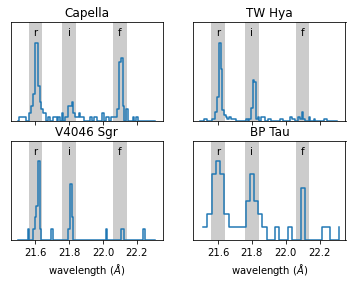
\includegraphics[width=0.49\textwidth]{figs/o7f2i.png}
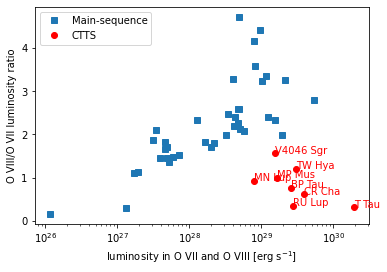
\includegraphics[width=0.49\textwidth]{figs/o72o8.png}
\caption{Signatures of accretion in classical T Tauri stars from high-resolution grating spectroscopy. \emph{Left:} Density-sensitive O~{\sc vii} triplet. Capella is a main-sequence star with an $f/i\sim 4$, while the other three sources are examples of CTTS with $f/i < 1$. All lines are unresolved, they appear wider in BP~Tau because the data is taken with a lower-resolution spectrograph (Chandra/LETG, while the other three are Chandra/HETG). \emph{Right:} Ratio of O~{\sc viii} to O~{\sc vii} line flux compared to the total flux in oxygen lines. All accreting sources are well offset from the main-squence stars, indicating additional soft emission plasma. Modified from Ref.~ \cite{2013ApJ...771...70G} (see there for data sources). \label{fig:softexcess}}
\end{figure}


Second, a lower O~{\sc viii}/O~{\sc vii}-ratio is another feature that sets CTTS  apart from WTTS, their non-accreting sibblings (see Fig.~\ref{fig:softexcess} right). This indicates that the X-ray emission in CTTS is produced by an, on average, cooler plasma compared to non-accreting stars of comparable luminosity\footnote{Non-accreting stars show a correlation between plasma temperature and X-ray luminosity so that one must correct for this to find any accretion-driven effect in plasma temperature.} \cite{2007A&A...473..229R,2007A&A...474L..25G}. Another way of reading this figure is that 
CTTS have an intrinsic (coronal) O~{\sc viii}/O~{\sc vii}-ratio in line with low-luminosity WTTS or main-sequence stars since fainter coronae are also cooler. This view implies that CTTS have additional cool plasma compared to normal corona, and this additional plasma may be accretion-powered as the expected temperature of the post-shock plasma radiates strongly in O~{\sc vii} and not in O~{\sc viii}.

A third observation is that CTTS usually show abundances that are Ne enhanced and Fe depleted compared to solar abundances \citep{Stelzer_2004}. This pattern is also seen in active stars, where it is attributed to element separation in the corona due to different values of the first ionization potential (FIP) of ions. Neon has a particularly high FIP and iron a particularly low one, so the pattern observed is called IFIP (inverse FIP). However, CTTS are cooler than main-sequence stars of comparable luminosity and so alternative scenarios have been discussed \citep{Drake_2005}. Since accretion comes from the inner edge of the accretion disk, it is possible that disk processes separate elements. If gain-forming elements condense into grains, pebbles, and proto-planets, the material on the inner disk edge might be depleted of Fe, Si, and similar metals, while noble gases stay in the gas phase and are thus preferentially accreted. 

Fourth, X-ray grating spectra of TW Hya have sufficient S/N to determine  line shifts for some strong emission lines. The lines from cooler plasma show a $38.3 \pm 5.1$~km/s shift compared with the hotter, coronal lines \cite{2017A&A...607A..14A}. And while this indicates different origins for the cool and hot plasma, it is also much less than the free-fall velocity. This implies that we must see the shock almost perpendicular to the line-of-sight. TW~Hya is observed close to pole-on, so the accretion shock(s) seen in X-rays must the located in the equatorial region for TW~Hya.




\subsection{Physics of accretion in 1D}
\label{sect:accretionphysics}
With X-ray observations pointing to a different emission pattern in accreting stars compared to non-accreting ones, we discuss simple models to check if these X-ray signatures are broadly compatible with X-ray emission from the accretion shock.

Many aspects of the accretion physics can be described in a 1D model where all mass motion is parallel to the magnetic field lines. We review some of the basic physics of accretion columns and accretion shocks. While modern models go far beyond such a simple prescription, the foundation of all accretion shock models still is to convert the gravitational energy in the disk to kinetic energy of the free-falling gas, which in turn gets turned into heat and radiation in the accretion shock.

The free fall velocity $v_{\textnormal{free}}$ of material coming from an inner disk radius of $R_\mathrm{in}$ onto a star with mass $M_*$ and radius $R_*$ is
\begin{equation}
v_{\textnormal{free}} = \sqrt{{2GM_*} \left(\frac{1}{R_*} - \frac{1}{R_\mathrm{in}}\right)} \approx 620 \sqrt{\frac{M_*}{M_\odot}}\sqrt{\frac{R_\odot}{R_*}} \frac{\textnormal{km}}{\textnormal{s}}\ \label{eqn:freefall}
\end{equation}
where $G$ is the gravitational constant. The inner radius is typically a few stellar radii and thus $v_\textnormal{free}$ is very close to infall from infinity.


\subsubsection{The shock front}
We concentrate on stationary shocks and ignore all turbulent fluxes. In the shock front, ions and electrons are heated differently, but they remain strongly coupled and reach the same temperatures within a few mean-free path lengths---a region so thin that it is justified to treat them as a single fluid.

Somewhere along the accretion column, a shock forms when the forward ram pressure becomes comparable to the pressure of the underlying material. The shock front itself is very thin, only of the order of a few mean free paths \cite{raizerzeldovich}. Therefore it can be treated as a mathematical discontinuity described by the Rankine-Hugoniot jump-conditions \cite[][chap.~7, \S~15]{raizerzeldovich}; in the shock the super-sonic infall velocity is converted mostly into thermal energy. Since we assume the direction of flow parallel to the magnetic field, the Lorentz force does not influence the dynamics. Marking the state in front of the shock front by the index 0, that behind the shock by index 1, the Rankine-Hugoniot conditions become
\begin{eqnarray}
\rho_0 v_0 &=& \rho_1 v_1 \label{RH1}\\
P_0+\rho_0 v_0^2 &=& P_1+\rho_1 v_1^2 \label{RH2}\\
\frac{5 P_0}{2\rho_0}+\frac{v_0^2}{2}&=&\frac{5 P_1}{2\rho_1}+\frac{v_1^2}{2} \ ,\label{RH3}
\end{eqnarray}
where $v$ is the velocity, $\rho$ the total mass density of the gas and $P$ its pressure.

From the jump conditions, the shocks will heat gas to a temperature $T$
\begin{equation}
kT \simeq \frac{3}{16}\mu m_p v^{2} \approx 0.3\,{\rm keV}\left(\frac{v}{500\,{\rm km/s}}\right)^{2} \approx3.5\times10^6\,{\rm K} \left(\frac{v}{500\,{\rm km/s}}\right)^{2},
\label{eqn:Tshock}
\end{equation}
where $\mu$ is the dimensionless atomic weight.

\subsubsection{Structure of the post-shock region}

In the post-shock region the gas emits radiation and cools down, so the energy of the gas is no longer conserved.  However, the particle number flux $j$ of ions (and atoms)
\begin{equation}j=nv\label{j_n}\end{equation}
is conserved, where $n$ is the ion/atom number density; the electron number density is denoted by $n_{\mathrm{e}}$. The total momentum flux $j_p$ is conserved, since we ignore the momentum loss by radiation:
\begin{eqnarray}
j_p&=&\mu m_{\mathrm{H}} n v^2+P \nonumber \\
   &=&\mu m_{\mathrm{H}} n v^2+nkT \label{j_p}
\end{eqnarray}
where $m_{\mathrm{H}}$ denotes the mass of a hydrogen atom.

Let us next consider the energy balance in the post-shock region. In general,
\begin{equation} \label{tsminuspdvisdu} T d\Sigma -P dV=dU \end{equation}
where $\Sigma$ denotes the entropy and $U$ the internal energy of the plasma. The quantity $T d\Sigma=dQ$ denotes the heat flux through the boundaries of the system. Here, the energy loss $Q_{col}$ proceeds through collisionally excited higher electronic states, which decay radiatively.

Assuming that the shock location is stationary, we get $\frac{d}{dt}=\frac{\partial}{\partial t}+\frac{\partial z}{\partial t}\frac{\partial}{\partial z}=v\frac{\partial}{\partial z}$ depending on the location $z$, measured from the shock front inwards; differentiation with respect to $z$ will be indicated by $'$.
The internal energy $U$ is in this case the thermal energy $U=\frac{3}{2}kT$, the pressure $P$ can be rewritten using the equation of state. The specific volume $V$ is the inverse of the number density $V=\frac{1}{n}$.
It is convenient to write the electron number density as \mbox{$n_{\mathrm{e}}=x_e n$,} with $x_e$ denoting the number of electrons per heavy particle so that Eq.~\ref{tsminuspdvisdu} becomes
\begin{equation}
\label{energyelec}
v\left(\frac{3}{2}x_e k T_{\mathrm{e}}\right)'+v x_e n k T_{\mathrm{e}} \left(\frac{1}{n}\right)'=-Q_{col} x_e n\,.
\end{equation}

We now have $n$, $v$, and $T$ as variables and three hydrodynamic (HD) equations (\ref{j_n}, \ref{j_p}, and \ref{energyelec}), so the structure of the post-shock region can be calculated.

Simulations based on these or very similar formulas show that the accretion shock produces plasma matching the observed X-ray temperatures \citep{lamzin_1998} and the total energy in the accretion stream can be determined from fitting UV and optical spectra to determine the mass accretion rate \citep{calvet_1998}. Observations of the density-sensitive line ratios in He-like triplets such as in Fig~\ref{fig:softexcess} (left) can be explained by 1D models assuming a combination of accretion shock and coronal plasma \cite{Guenther_2007} and at the same time give a mass accretion rate that can be compared to observations of UV and optical tracers.


{\color{red} TBD: Some numbers?}

\subsection{Why we need to go beyond 1D models}
One dimensional models are successful in many aspects, but there are also observational and theoretical arguments suggesting that important physical processes are not captured in 1D. In deep Chandra observations of TW~Hya, densities can be measured in three density-sensitive triplets covering a range of peak formation temperatures. The density is highest in Mg~{\sc xi} and lowest in O~{\sc vii}, although Mg~{\sc xi} is formed at a higher temperature \cite{Brickhouse_2010}. Because the post shock region is isobaric, one would expect Mg~{\sc xi} emission from a region directly behind the accretion shock and O~{\sc vii} from denser layers deeper down ($P\propto T$). One possible explanation is that the observed O~{\sc vii} emission is not from the accretion shock itself, but originates in hot material that escapes the accretion column to the side and is denser than a normal stellar corona, but not as dense as plasma immediately behind the accretion shock. That in turn means that the O~{\sc vii} flux may not be a good measure of the total accretion rate even when corrected for coronal contributions.

This is corroborated by the surprising observation that X-ray determined mass accretion rates are very similar for most sources despite a difference in optically determined mass accretion rate by three orders of magnitude \cite{2011A&A...526A.104C} which can be explained if the accretion streams are not homogeneous structures but have a density profile and the inner layers either form shocks deeper in the atmosphere or simply have their X-ray emission reprocessed by the outer layers of the accretion stream \cite{Sacco_2010,Schneider_2018,2021Natur.597...41E}.

Time variability can give us further insight. In V4046~Sgr the emission lines from soft, presumably shock-heated, plasma have a period of exactly half the orbital period of the close binary. Together with Doppler-imaging this leads to the interpretation that we can observe the shock only when the accretion flow is perpendicular to the line of sight, while the accretion funnel blocks the view of the shocked region at other times \cite{2012ApJ...752..100A}. 
% Similarly, the accretion funnel has been observed to block the X-rays from AA~Tau for certain rotational phases. This includes coronal and accretion generated X-rays \cite{2007A&A...462L..41S,2007A&A...475..607G}.
There are several classes of variable pre-main sequence accretors, including FU~Ors and EX~Ors, where the accretion rate changes by orders of magnitude or stars where a change in the disk structure moves absorbing material into our light of sight, such as in RW~Aur or also in AA~Tau. However, those changes happen on much larger scales than the accretion shock itself and are not discussed here any further.


Observations of our Sun provide the opportunity to look for situations analogous to accretion onto young stars, although the accretion rate would be obviously much lower. The benefit of such data is that spatially resolved data in the UV and EUV, even if not in X-rays, are available with long time coverage and high cadence while most observations of the accretion shock on young stars are spatially unresolved. One particularly interesting observation is the event that happened on June, 7$^{th}$, 2011 when parts of an erupting filament fell back into the Sun \cite{2013Sci...341..251R} (see also \cite{Reale_2014}). The infall speed of up to 450~km/s was comparable to free-fall accretion onto T Tauri stars and the initial infall triggered upflows that shocked with later fragments causing UV emission on the Sun; such a process would not be covered in a 1D approach.



A correct description of the coupling between radiation and hydrodynamics is necessary to account for the effects of absorption and emission of radiation, because photons and mass may travel differently through the domain. Indeed, improved models including local thermodynamic equilibrium (LTE) radiation transfer now show that the heated photosphere does not radiate as a simple black body in the optical and infrared \cite{Dodin_2012,Dodin_2013}, but also produces line emission, which selectively fills in some photospheric absorption lines, possibly biasing accretion rate measurements based on optical veiling.
Similar optical depth effects also
have a non-negligible effect on the typical characteristics of the 
accretion dynamics, on the estimation of its X-ray surface luminosity 
\cite{Sa_2019}, on the heating of the accretion column \cite{1999AstL...25..430L,Costa_2017}, and the predicted lightcurve \cite{2021ApJ...908...16R}. Thus, we now turn to the 3D structure of the accretion process.

\subsection{The multi-D structure of the accretion shock}

\begin{figure}[t]
    \centering
    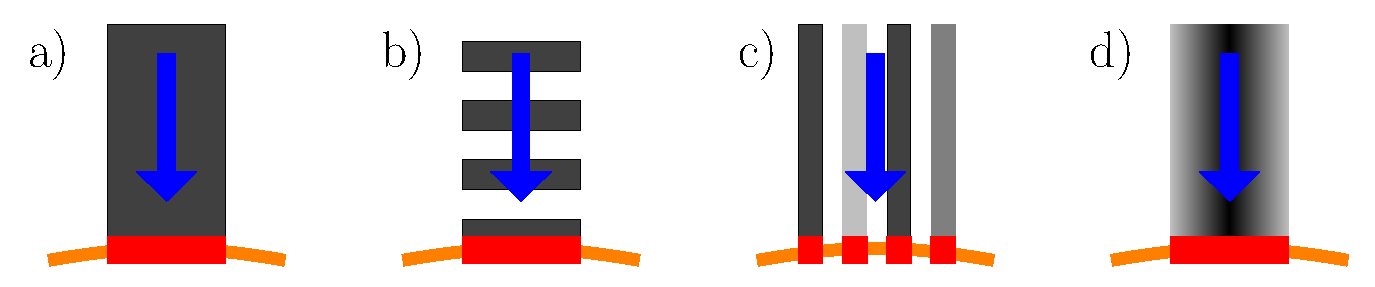
\includegraphics[width=11cm]{sketches/column_sketch.pdf}
    \caption{Different models proposed for the 
    structure of accretion columns. The~stellar surface is at the bottom (orange) and 
    material flows along a magnetic field line onto the stellar surface (indicated 
    by the blue arrow). The~accretion shock (red) forms on the stellar surface. 
    Density is shown as gray scale. From left to right: 
    a) One homogeneous column with one density and a single infall velocity; 
    b) one ``column'' is decomposed into individual blobs that are, individually, homogeneous in density;
    c) multiple columns that are individually homogeneous, i.e.,~have different densities but are otherwise equal; 
    d) one column with a density stratification (high density in the center of the column indicated by the black region, lower density in the outer region indicated by the grayish color) and one infall velocity. 
    }
    \label{fig:column}
\end{figure}

The 3D density structure of the accretion columns is key to correctly describe accretion and 
different scenarios have been proposed (see Fig.~\ref{fig:column}). The first models considered one homogeneous column with one density and a single infall velocity (Fig.~\ref{fig:column}\,a). 
\citet{Orlando_2010, Orlando_2013} modelled a constant and uniform accretion stream that propagates along the magnetic field lines considering uniform  (see upper panels in Fig.~\ref{fig:accretion}) and nonuniform  (see lower panels in Fig.~\ref{fig:accretion}) stellar magnetic fields at the impact region of accretion columns. In these models, the plasma follows the magnetic field lines and impacts onto the chromosphere, forming a hot slab at the base of the accretion stream with temperatures up to $\approx 5\times10^6$~K (see Fig.~\ref{fig:accretion}). After impact, part of the shock column is buried under a column of optically thick material and may suffer significant absorption \cite{Orlando_2010,Orlando_2013}.
The structure, dynamics and stability of the accretion shock strongly depend on the configuration and strength of the magnetic field \cite{Orlando_2010}, and thus on the plasma $\beta$ defined as $\beta =$~gas pressure/magnetic pressure. 
The post-shock region is efficiently confined by the magnetic field for shocks with $\beta \lesssim 1$, while strong outflows of shock-heated material 
escape laterally for shocks with $\beta$ above $10$ \cite{Orlando_2010,Orlando_2013}. For intermediate cases (see left upper panel in Fig.~\ref{fig:accretion}), the escaping material is kept close to the accretion column 
if the magnetic field is strong enough and gradually surrounds the primary stream until it eventually perturbs the accretion column (see right upper panel in Fig.~\ref{fig:accretion} and \cite{Orlando_2010}). 
A nonuniform magnetic field causes a large field component perpendicular to the stream velocity, and the resulting additional magnetic pressure at the base of the stream limits the plunging of the slab into the chromosphere (see left lower panel in Fig.~\ref{fig:accretion}) and rather pushes chromospheric material sideways along the magnetic field lines to the upper atmosphere (see right lower panel in Fig.~\ref{fig:accretion} and \cite{Orlando_2013}). 

\begin{figure}[t]
    \centering
    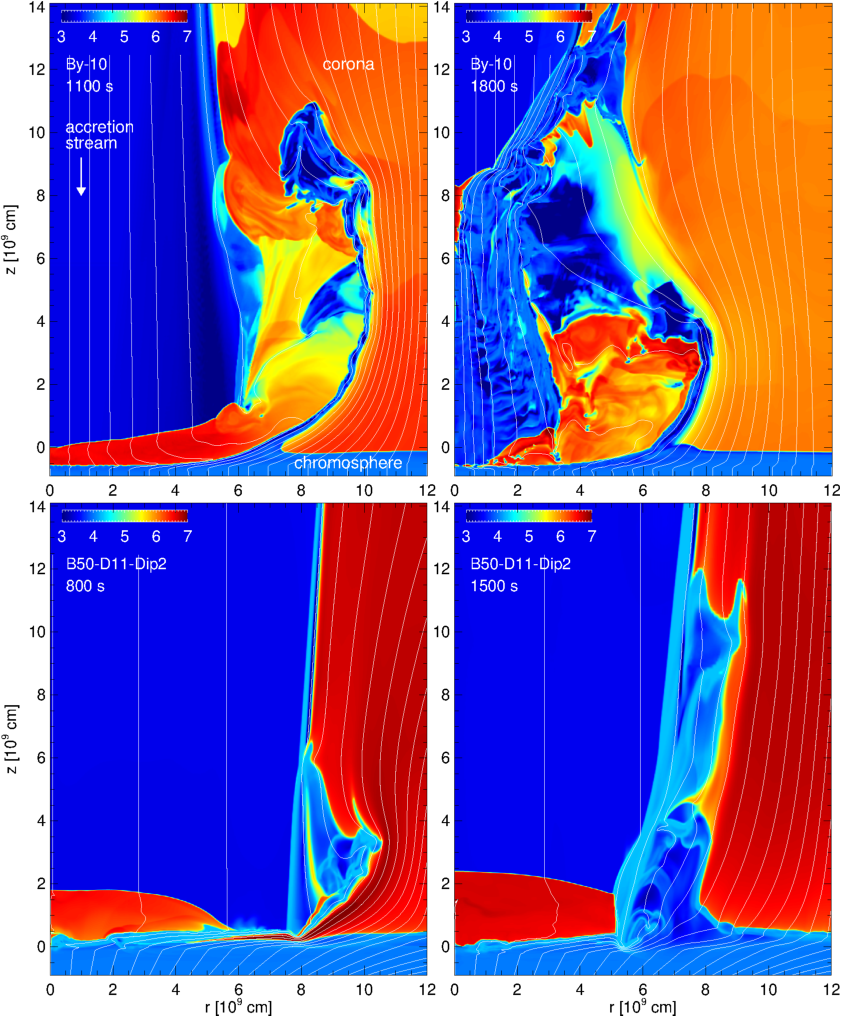
\includegraphics[width=9cm]{figs/accretion.pdf}
    \caption{Temperature distributions in the ($r$, $z$) plane in log scale at the labeled times (increasing from left to right) for two different models: simulation By-10 from \cite{Orlando_2010} (upper panels), and simulation B50-D11-Dip2 from \cite{Orlando_2013} (lower panels). The initial position of the transition region between the chromosphere and the corona is at $z = 0$. The white lines mark magnetic field lines. Figure courtesy of S. Orlando.}
    \label{fig:accretion}
\end{figure}

\begin{figure}[t]
    \centering
    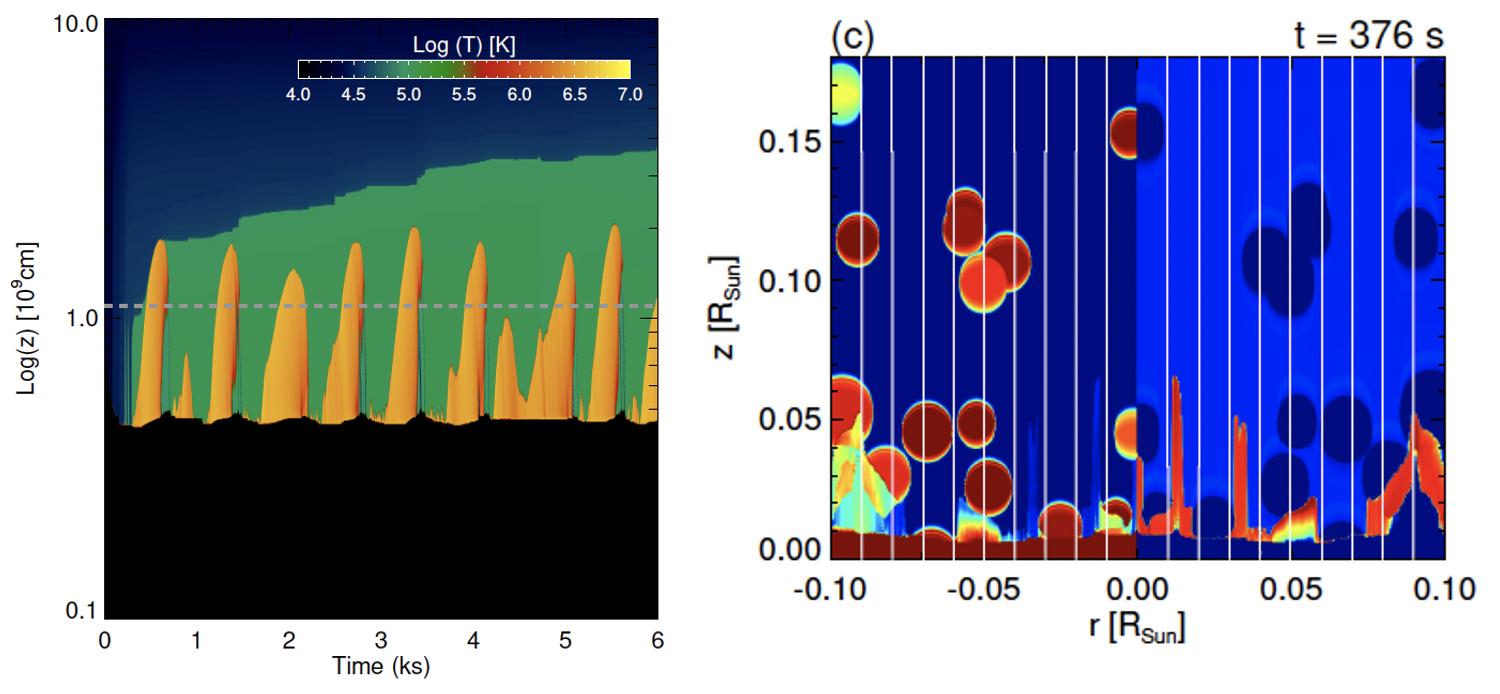
\includegraphics[width=12cm]{figs/colombo.png}
    \caption{\emph{Left:} Color maps of evolution of density (left half-panel) and temperature (right half-panel) of plasma for the general case of fragmented stream explored in \cite{Colombo_2016}. White lines represent magnetic field lines. Figure adapted from \cite{Colombo_2016}. 
    \emph{Right:} Space-time map, in logarithmic scale, of temperature for the non-LTE model run by \cite{Colombo_2019b}. The green region in the
    bottom panel corresponds to the hottest part of the precursor. The gray
    dotted lines in both panels mark the pre-impact position of the 
    chromosphere. Figure adapted from \cite{Colombo_2019b}.}
    \label{fig:colombo}
\end{figure}

{\color{red} TBD: Change following sentence into a motivation for more complex simulations}
More complex accretion streams are modelled with multi-D MHD simulations, too. Examples are density stratification and clumpy structures formed by several blobs (Fig.~\ref{fig:column} c \& d and, e.g., \cite{Matsakos_2013,Colombo_2016}). Perturbations in the accretion column (namely a clumpy stream and a oblique impact) can disrupt the shock structure and create a more inhomogeneous post-shock region with the post-shock region still strongly dependent on the plasma $\beta$ \cite{Matsakos_2013}.
Randomly fragmented accretion streams (see left panel in Fig.~\ref{fig:colombo}) produce reverse shocks that propagate upflows through the unshocked fragmented stream when the blobs impact onto the stellar chromosphere \cite{Colombo_2016}.
As a result, the structure of the post-shock region is very complex and consists of several knots and filaments of plasma with a wide range of velocities, densities, and temperatures \cite{Colombo_2016}.

Simulations now also include absorption by pre-shock material {\color{red} to explain TBD}. An envelope of dense and cold material may develop around the shocked column, influencing the observability of the shock-heated plasma in the X-ray band (\citep{Orlando_2013}, see also Fig.~\ref{fig:accretion}). The X-ray emission from the shocked region can be heavily reduced due to the absorption by  optically thick material around the hot plasma. The magnitude of this effect depends on the distribution of material along the line of sight towards the shock \cite{Bonito_2014}. A model using radiative transport in the non-LTE regime devoloped by \cite{Colombo_2019b} estimated that about $\approx 70$\% of the radiation emitted by the post-shock plasma is absorbed by the pre-shock accretion column, forming a radiative precursor of the shock (green region in right panel of Fig.~\ref{fig:colombo}).

In addition to MHD models, laboratory experiments are now available, which can be scaled to accretion shocks on CTTS since the MHD equations are invariant under certain scaling transformations. Nowadays, laboratory experiments employ magnetic fields, densities, temperatures, and other hydrodynamical parameters that can be scaled to the stellar case. 
One example of such an experiment consisted of a collimated narrow laser-produced plasma stream that propagates along a strong external magnetic field, very similar to accretion on CTTS \cite{Revet_2017}. Similarly to the MHD simulations described above, the laboratory experiment shows
that, upon impact, the plasma is ejected laterally from the accretion shock and then refocused by the magnetic field towards the incoming stream, forming a shell that envelops the shocked core \cite{Revet_2017}. This hot shell provides an additional absorber that reduces the observable  X-ray emission. Also, experiments with accretion streams impacting a tilted surface have been performed, which correspond to accretion stream along complex magnetic field structures. The resulting plasma flows is highly asymmetric and a large amount of plasma escapes laterally from the accretion flow, showing poor confinement of the accreted material and reduced heating compared to the normal
incidence case \cite{Burdonov_2020}.

\subsection{Variability and accretion outbursts}
In the previous sections, we concentrated on CTTS with their well-ordered magnetically-funneled accretion streams. There are other classes of pre-main sequence accretors, but those are very rare and therefore hard to observe. One group are accretion outbursts, where the accretion rate suddenly jumps by several orders of magnitude and then decays back over time scales from months (EX~Or objects) to decades or centuries (FU~Or objects) \cite{2014prpl.conf..387A}. EX~Or outbursts are not only shorter, they can also be observed to be repetitive. These eruptive stars show bright and hot coronal emission, possibly because the coronal structures are compressed with a higher density or because having a bright corona in the first place somehow triggers the accretion burst \cite{2011ApJ...741...83T,2019ApJ...883..117K}. Most sources are highly absorbed, but soft emission compatible with an accretion shock has also been observed \cite{2010A&A...522A..56G}---again much brighter than in CTTS due to the increased accretion rate. 
On the other hand, in CTTS with their much lower accretion rates, we have no evidence of any correlation between magnetic flares and accretion events \cite{1997A&A...324..155G,2019ApJ...876..121E}.


\subsection{Towards a coherent picture of the accretion shock}
X-ray observations of CTTS show features unique to accreting stars, primarily a cool ($\sim10^6\,$K), high-density ($n_e\gtrsim10^{12}\,$cm$^{-3}$ plasma excess. This excess is compatible with expectations for a high-velocity shock, i.e., emission from the post-shock region of the accretion shock. However, uniform, homogeneous accretion columns produce a post-shock structure incompatible with the X-ray data: the measured density structure is opposite to the post shock region (Brickhouse+ 2010), the derived mass-accretion rates are too low, and the filling factor too large. Therefore, more complex accretion funnels are needed to reconcile observations with models. The leading idea is currently a density stratified or fragmented accretion stream, where the strength and configuration of the magnetic field plays an important role. Also, absorption by optically thick material and the effect of radiative heating of pre-shock material brings models closer to observations. In summary, a dynamic and structured accretion funnel is the most likely explanation for the observed emission as it naturally leads to a multitude of different emitting regions to reconcile observations.
